Im Folgenden wird der theoretische Hintergrund zum Experiment erläutert.
\subsection{Beschreibung von verlustbehafteten Leitungen}
Um die elektrischen Eigenschaften von Bauteilen zu Modellieren wird üblicherweise ein Ersatzschaltbild verwendet. Abbildung \ref{fig:Ersatzschaltbild} zeigt die Ersatzschaltbilder für eine verlustfreie und eine verlustbehaftete Leitung. Die Bausteine werden in diesem Fall als \textit{Beläge} bezeichnet: Kapazitätsbelag $C$, Induktivitätsbelag $L$, ohmscher Belag $R$, Querleitfähigkeitsbelag $G$. Es wird zudem zwischen Längsspannungsverlust (an $R$) und Querstromverlust (an $G$) unterschieden, wobei die ohmschen bzw. Längsspannungsverluste meist überwiegen.
\begin{figure}[h!]
	\centering
	\begin{subfigure}[t]{0.35\textwidth}
	\centering
\begin{circuitikz}
	\draw (-.5, 0)
	to[american inductor, l = $L$] (2.5, 0)
	to (3.5, 0);
	\draw (-.5, -2)
	to (3.5,-2);
	\draw (2.5,0)
	to[C, l = $C$] (2.5,-2);	
\end{circuitikz}
\subcaption{}
\label{fig:OhneVerlust}
\end{subfigure}
\begin{subfigure}[t]{0.55\textwidth}
	\centering
\begin{circuitikz}
	\draw (-.5, 0)
	to[R, l = $R$] (2.5,0)
	to[american inductor, l = $L$] (3.5, 0)
	to (7, 0);
	\draw (-.5, -2)
	to (7,-2);
	\draw (4.5,0)
	to[R, l = $G$] (4.5,-2);
	\draw (6,0)
	to[C, l = $C$] (6,-2);	
\end{circuitikz}
\subcaption{}
\label{fig:MitVerlust}
\end{subfigure}
	\caption[Ersatzschaltbilder]{Ersatzschaltbilder einer verlustfreien (\ref{fig:OhneVerlust}) und einer verlustbehafteten Leitung (\ref{fig:MitVerlust})}
	\label{fig:Ersatzschaltbild}
\end{figure} \\
Mit Hilfe des Ersatzschaltbildes für die verlustbehaftete Leitung kann die Telegrafengleichung
\begin{align}
	\pdv[2]{U}{t} = LC\pdv[2]{U}{x} + (LG + RC)\pdv{U}{x} + RGU
\end{align}
für die Spannung $U(x,t)$ abgeleitet werden. Ihre Lösung ist
\begin{align}\label{eq:LosungTelegraph}
	U(x,t) = U_0 \exp(-\gamma x)\exp(i\omega t) \quad ,
\end{align}
hierbei ist $\omega$ die Frequenz der Spannung und $\gamma = \alpha + ik = \sqrt{(R+i\omega L)(G+i\omega C)}$\footnotemark die Ausbreitungskonstante. Sie enthält den Dämpfungsbelag $\alpha$ und den Phasenbelag $k$ (die Wellenzahl).
\footnotetext{In Polarschreibweise: $\gamma = \sqrt[4]{(R^2+\omega^2L^2)(G^2+\omega^2C^2)}\exp(\frac{i}{2}\left(\atan(\frac{\omega L}{R})+\atan(\frac{\omega C}{G})\right))$.} \\
Durch Dispersion kann es zur Verzerrung des Signals kommen, entscheidend dabei sind der Aufbau und der Wellenwiderstand $Z_0$ des Kabels. Für ein harmonisches Signal in einem Kabel mit gleichbleibender Geometrie gilt
\begin{align}
	Z_0(\omega) = \frac{U(\omega)}{I(\omega)} = \sqrt{\frac{R+i\omega L}{G+i\omega C}} \quad .
\end{align}
In einem verlustlosen Kabel tritt keine Dispersion und damit auch keine Verzerrung auf, da die  Phasengeschwindigkeit
\begin{align*}
	v = \lim\limits_{R,G\rightarrow 0}\frac{\omega}{k} = \frac{\omega}{\sqrt[4]{\omega^4L^2C^2}\sin(\frac{\pi}{2})} = \frac{1}{\sqrt{LC}}
\end{align*}
konstant ist.

\subsection{Überlagerung von Signalen}
Abbildung \ref{fig:Schema} zeigt wo sich die Spannungsabfälle in einer vollständigen, d.h. geschlossenen, Schaltung befinden. Jede Störstelle, d.h. jede Art von Übergang, in der Schaltung wirkt reflektierend. Der Reflexionsfaktor
\begin{align}\label{eq:Reflexion}
	\Gamma = \frac{U_\text{r}}{U_0} = \frac{Z_\text{A}-Z_0}{Z_\text{A}+Z_0}\quad \footnotemark
\end{align}
gibt dabei den Grad der Reflexion an.
\footnotetext{Im Zähler wurde verwendet, dass die am Abschlusswiderstand abfallende Spannung die Überlagerung von Eingangs- und reflektiertem Impuls ist: $Z_\text{A}I = U_\text{A} = U_\text{r}+U(x) = U_\text{r}+Z_0I$. Im Nenner wird aus Abbildung \ref{fig:Schema} abgelesen, dass $U_0 = U(x)+U_\text{A} = I(Z_0+Z_\text{A})$.}
Bei $Z_\text{A} = Z_0$, findet keine Reflexion statt, die Leitung ist \textit{angepasst}.
Die Spannung des reflektierten Signals kann mit einer Laplace-Transformation
\begin{align}
	U_\text{r}(x,t) = \mathcal{L}^{-1}\{U_\text{r}(p,t)\} = \mathcal{L}^{-1}\{\Gamma(p)U_\text{h}(p,t)\}
\end{align}
berechnet werden, wobei $U_\text{h}(p,t)$ der Eingangspuls und $\Gamma(p) = \frac{Z_\text{A}(p)-Z_0}{Z_\text{A}(p)+Z_0}$ der Reflexionskoeffizient im Impulsraum sind.\footnotemark \
\footnotetext{Im Impulsraum gilt für den Abschlusswiderstand $Z_\text{A} = R$, bei einem ohmschen Widerstand, $Z_\text{A} = pL$ bei einer Induktivität und $Z_\text{A} = \frac{1}{pC}$ bei einer Kapazität.}\todo{QUELLE}
Die resultierende Spannung $U_\text{r}(x,t)$ enthält eine Exponentialfunktion der Form $\exp(-t/T)$, in der die Zeitkonstante $T$ enthalten ist. Zwischen ihr und der Signalspannung $U(x,t)$ besteht ein direkter Zusammenhang, der in Abbildung \ref{fig:Zeitkonstanten} dargestellt ist.
\begin{figure}[h]
	\centering
	\begin{circuitikz}
	\draw[latex'-latex'] (1.5,-2.5) -- (5.5,-2.5) node[below, xshift=-2cm] {$x$};
	\draw[dashed] (1.5,-2.1) -- (1.5,-2.4);
	\draw[dashed] (5.5,-2.1) -- (5.5,-2.4);
	\draw (-.5, 0)	to (7, 0);
	\draw (-.5, -2)	to (7, -2);
	\draw (0,0)	to[sinusoidal voltage source, l = $U_g$] (0,-2)	to (0,-2);
	\draw[latex'-latex'] (1.5,-0.1) to (1.5,-1.9) node[right, yshift=+0.9cm] {$U_0$};
	\draw[-latex] (5.5,-.1) -- (5.5,-1.9) node[right, yshift=+0.9cm] {$U(z)$};
	\draw (7,0)	to[R, l = $Z_\text{A}$] (7,-2);
	\draw[dashed] (7.1,0) to (8,0);
	\draw[dashed] (7.1,-2) to (8,-2);
	\draw[latex'-latex'] (8,-0.1) to (8,-1.9) node[right, yshift=+0.9cm] {$U_\text{A}$};
\end{circuitikz}
	\caption{Schematische Darstellung einer Schaltung mit Abschlusswiderstand zur Veranschaulichung der Spannungsabfälle}
	\label{fig:Schema}
\end{figure} \\
Wenn sich mehrere Störstellen in einer Schaltung befinden, wird der Spannungspuls auch mehrfach reflektiert. Es könnte beispielsweise eine Störstelle am Anfang und eine am Ende der Leitung mit den Reflexionskoeffizienten $\Gamma_\text{A}$ und $\Gamma_\text{E}$ geben. Ist die Eingangsspannung $U_0$, dann ist die Spannung des reflektierten Pulses nach der ersten Reflexion am Leitungsende $U_1 = \Gamma_\text{E}U_0$. Dieser Puls wird wiederum an der Störstelle am Leitungsanfang reflektiert, der hier reflektierte Puls hat die Spannung $U_2 = \Gamma_\text{A}U_1 = \Gamma_\text{A}\Gamma_\text{E}U_0$ usw. Der reflektierte Puls nach $n$ Reflexionen hat demnach die Amplitude
\begin{align*}\label{eq:Un}
	U_n = \begin{cases}
		\left(\Gamma_\text{A}\Gamma_\text{E}\right)^\frac{n}{2}U_0 &\quad, \text{ falls $n$ gerade} \\
		\left(\Gamma_\text{A}\Gamma_\text{E}\right)^\frac{n-1}{2}\Gamma_\text{E}U_0 &\quad, \text{ falls $n$ ungerade}
	\end{cases} \quad.
\end{align*}
Die Gesamtspannung $U_\text{ges}$ ist die Überlagerung aller Impulse, also
\begin{align}
	U_\text{ges} &= U_0\sum_{n =0}^{\infty}\left(\Gamma_\text{A}\Gamma_\text{E}\right)^n + U_0\Gamma_\text{E}\sum_{n = 0}^{\infty}\left(\Gamma_\text{A}\Gamma_\text{E}\right)^n \notag \\
	&= U_0\frac{1+\Gamma_\text{E}}{1-\Gamma_\text{A}\Gamma_\text{E}} \quad,
\end{align}
wobei die geometrische Reihe verwendet wurde. Da der Puls eine bestimmte Zeitspanne $T$ benötigt um die Strecke vom Anfang bis zum Ende zurückzulegen, stellt sich der Grenzwert erst nach einiger Zeit ein. Das wird in Abbildung \ref{fig:ZeitlicherVerlauf} dargestellt.
\begin{figure}[h]
	\centering
	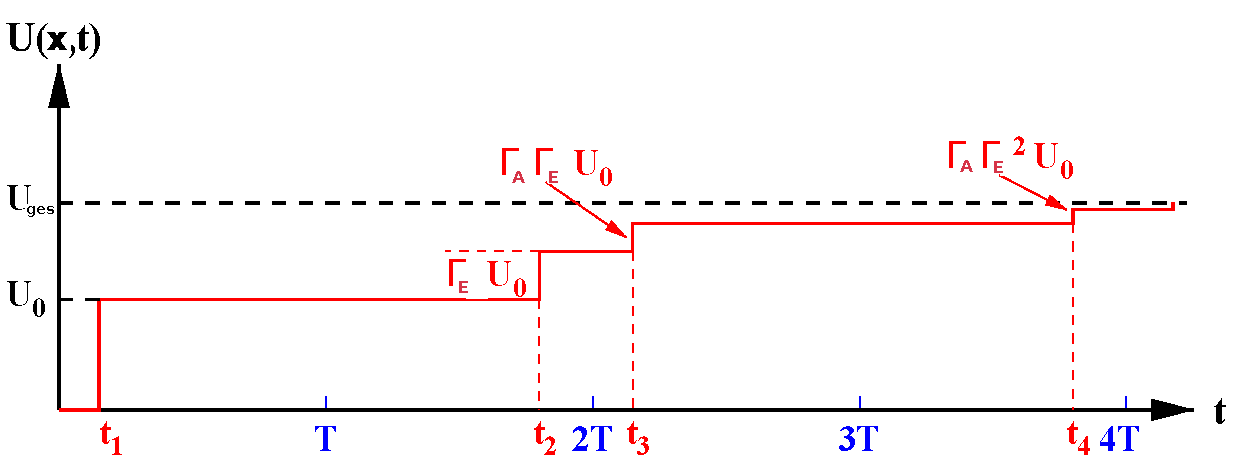
\includegraphics[width=0.6\textwidth]{Verlauf.pdf}
	\caption[Zeitlicher Verlauf der Signalspannung]{Zeitlicher Verlauf der Signalspannung $U(x,t)$ an einem festen Ort $x=ct_1$ \cite{E2}}
	\label{fig:ZeitlicherVerlauf}
\end{figure}

\subsection{Koaxialkabel}
Im Experiment werden Koaxialkabel verwendet. Sie bestehen aus zwei ineinander steckenden zylinderförmigen Leitern. Das Verhältnis der beiden Durchmesser bestimmt maßgeblich den Wellenwiderstand $Z_0$, den Längsspannungsverlust $R$ und den Querstromverlust $G$. Eine der Quellen dieser Verluste ist bei einem Koaxialkabel der \textit{Skin-Effekt}, d.h. das Verdrängen des Stroms aus dem Leiterinneren nach außen. Er wird dadurch verursacht, dass sich im Inneren des Leiters durch die Wechselspannung Wirbelfelder ausbilden, die den Wechselstrom wiederum nach außen verdrängen. Dieser Effekt ist bei hohen Frequenzen stärker, sodass $R$ und $G$ bei über \SI{100}{\kilo\hertz} nicht mehr frequenzunabhängig sind, sondern mit $\sqrt{\omega}$ ansteigen. \\
Für die Leitungskonstanten eines Koaxialkabels gelten die folgenden Beziehungen:
\begin{align}\label{eq:Theorie}
	R &= \frac{\sqrt{\frac{\pi\nu\mu_c}{\omega\Im{\varepsilon}}}}{2\pi}\left(\frac{1}{d}+\frac{1}{D}\right) \\
	&= \frac{\sqrt{\pi\rho\mu f}}{\pi}\left(\frac{1}{d}+\frac{1}{D}\right) \text{Die ist aus einer Quelle im Internet.} \\
	&= \sqrt{\frac{\mu f}{\sigma\pi}}\left(\frac{1}{d}+\frac{1}{D}\right) \\
	L &= \frac{\mu}{2\pi}\ln(\frac{D}{d}) \\
	G &= \frac{2\pi\sigma}{\ln(\frac{D}{d})} \\
	C &= \frac{2\pi\varepsilon}{\ln(\frac{D}{d})}
\end{align}
Hierbei sind $\varepsilon$ die Permittivität, $\mu$ die Permeabilität, $\sigma$ die spezifische Leitfähigkeit und $\rho$ der spezifische Widerstand.
\begin{figure}[h]
	\centering
	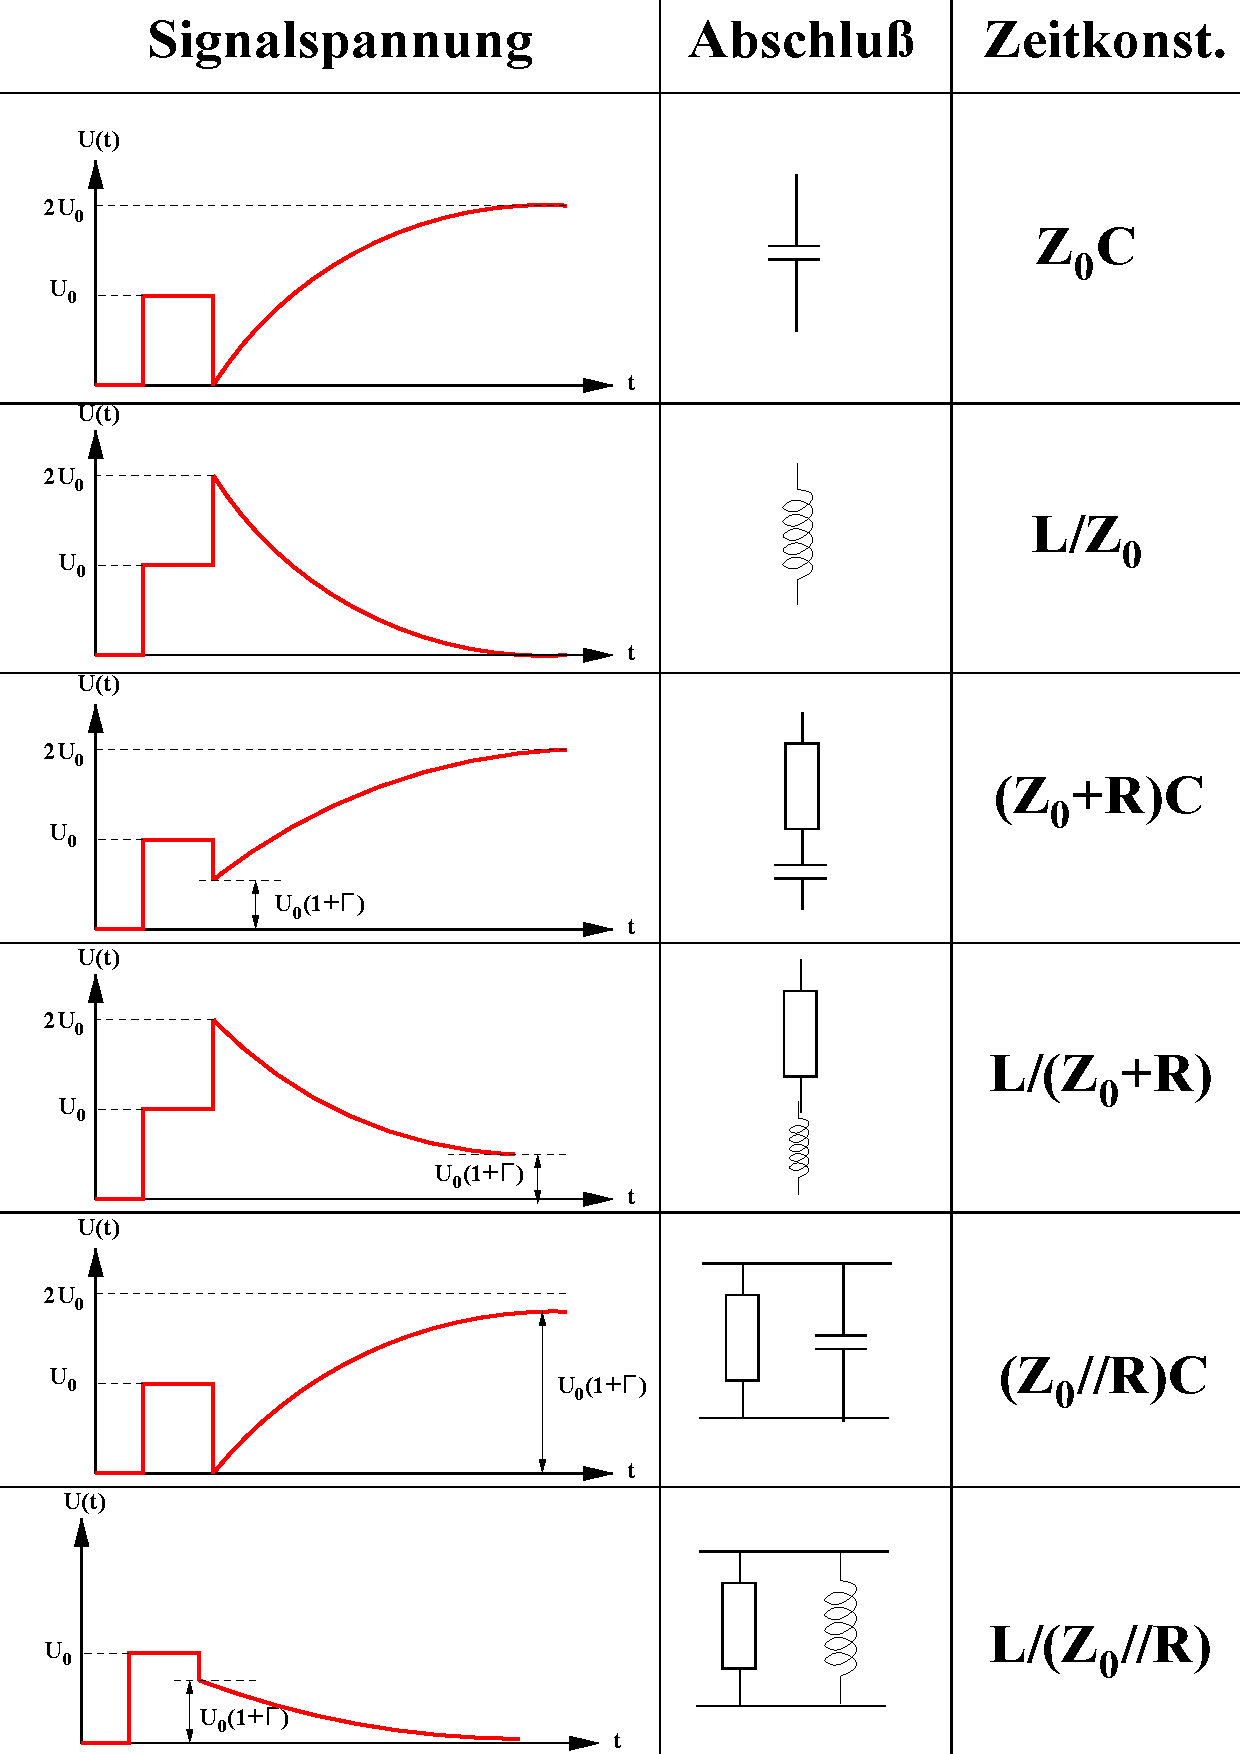
\includegraphics[width=0.55\textwidth]{Zeitkonstante.pdf}
	\caption{Signalspannung $U(x,t)$ und Zeitkonstanten für verschiedene Abschlusswiderstände \cite{E2}}
	\label{fig:Zeitkonstanten}
\end{figure}